\begin{table}[H]\centering\small
\begin{tabular}{@{}lrrrrr@{}}\toprule
Configuration & Accepted & Hosted seconds & Operations & Python calls & Complete cost \\ \midrule
U & 4/4 & 366.09 & 13 & 8 & Unknown \\
E & 4/4 & 390.90 & 16 & 10 & Unknown \\
E+ & 4/4 & 383.30 & 14 & 8 & Unknown \\
Conventional & 4/4 & Not matched & Not matched & Not matched & Unknown \\
\bottomrule\end{tabular}
\caption{Observed scientific campaign after all three recipients froze. Both request variants pass. Conventional construction was separate; its local function runtime is not compared with a hosted construction turn.}
\end{table}
The observed E--U and E+--E acceptance differences are both zero percentage points. No final mission fails. All logged Python executions exit successfully; inspection calls are included in the execution count. U, E and E+ add ten, thirteen and twelve tests respectively, beyond the common smoke test. Their complete final packets and reports remain frozen. These tests do not create additional independent mission families.

\begin{figure}[H]\centering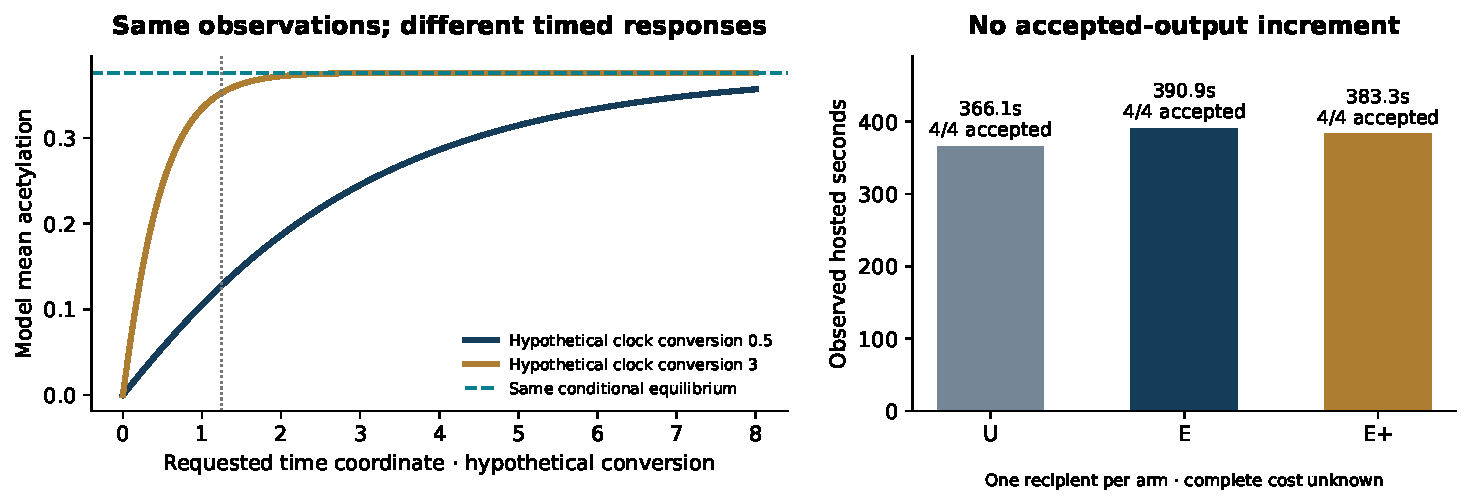
\includegraphics[width=0.97\linewidth]{figures/scientific_witness.pdf}\caption{Source-derived computational witness, not new biology. Clock conversions are hypothetical. At request time 1.25, the maximum state difference is 0.1433168 while the equilibrium agrees to numerical precision. The right panel reports single hosted observations, not a causal latency estimate.}\end{figure}
The accepted nominal model gives mean acetylation 0.3764225583 and a model spectral relaxation scale of 1.2815393182. Under the explicitly assumed conversion interval [0.4, 1.6] model units per minute, the propagated relaxation interval is [0.8009620739, 3.2038482954] minutes. It is a deterministic conditional interval, not measured biological timing or a confidence interval.

